%Reasoning over tabular data rarely happens in a single clean table. In realistic settings, relevant evidence is often distributed across multiple tables that differ in schema, layout, surface form, and numerical representation. As a result, question answering over tables is not only a matter of retrieving the right cell, but also of integrating heterogeneous evidence across tables, recovering implicit correspondences, and normalizing values before aggregation. These challenges are especially acute in high-impact domains such as healthcare and environmental decision-making, where data fragmentation and interoperability issues remain a persistent barrier to downstream use \citep{who,unep}.

%However, current benchmarks only partially capture this setting. Manual multi-table QA benchmarks are expensive to construct and difficult to scale, especially in domains where source data are private or inaccessible. Recent synthetic benchmark generation methods alleviate this bottleneck by automatically producing QA pairs from existing relational databases. Prior work has extended semantic parsing resources through templated multi-table SQL generation \citep{pal2023multitabqa}, used database constraints to create automatically verifiable reasoning questions \citep{oh2024erbench}, or synthesized increasingly complex SQL programs over structured table--text collections \citep{park2026sparta}. While effective, these approaches assume a clean relational regime: schemas are explicit, join paths are known, and the complexity of the generated questions is bounded by the structure of a pre-existing database.

%This assumption substantially limits the phenomena that can be evaluated. Real-world multi-table reasoning often involves \emph{non-relational} tables: tables with nested headers, merged columns, blank rows or columns, noisy cells, missing values, and other layout irregularities. Cross-table links may be \emph{implicit}, requiring semantic matching rather than explicit foreign-key joins. Moreover, analytical questions may require aggregation across a large number of parallel tables, sometimes under different units of measurement and numerical conventions. Existing generators do not directly target this regime, because they inherit both their schemas and their reasoning topology from an existing database.

%\mlc{aggiungere magari un esempio di query da inserire}

%We introduce \name, a flexible \emph{from-scratch} benchmark generator for numerical question answering over multiple non-relational tables. Unlike prior work, \name~ does not require an existing relational database, annotated examples, or manually curated source tables. Instead, a user specifies a target domain or topic together with lightweight generation controls, such as the number of attributes and attribute cardinalities. From this specification, \name~ first uses an LLM to generate a plausible schema and table metadata, including attribute semantics and candidate values. It then instantiates records combinatorially, guided by LLM-proposed intra-row and inter-row constraints that improve plausibility, executes templated SQL queries to obtain automatically verified scalar answers, and finally verbalizes the SQL into natural-language questions. \mlc{spiegazione dell'approccio deve essere migliorata, in base a come decidiamo di raccontarlo nel metodo}

%Starting from this generated relational source, \name~constructs challenging non-relational multi-table settings through controlled perturbations. We introduce structural perturbations that alter table layout (e.g., column merging, nested headers, blank rows/columns), cell-level perturbations that introduce realistic noise (e.g., distractor text, missing values, typos), and two multi-table reasoning regimes. In a \textbf{parallel} regime, the source table is horizontally partitioned into many subtables, each contributing one value to a global numerical aggregation; here, tables may also differ in units of measurement, requiring normalization before reasoning. In a \textbf{sequential} regime, the source table is vertically partitioned into a chain of subtables, and explicit join keys are masked with semantically equivalent but surface-divergent realizations, forcing models to recover implicit joins across tables. Because all benchmark instances originate from a single controlled source table, answer correctness remains automatically verifiable throughout.

%\mlc{inserire risultati}

%\mlc{altri possibili claim: focus sul fatto che l'utente possa generare su molteplici domini e topic; molteplici linguaggi; oppure maggiore focus sulla quantità di tabelle necessarie per ogni domanda (ne possiamo generare quante ne vogliamo); e generalmente sul fatto che l'utente può modificare il prompt di generazione iniziale, oppure aggiungere le sue perturbazioni, per customizzare come vuole il processo di generazione}

\section{Introduction}

The increasing digitization of structured data has made automatic information extraction and reasoning tools increasingly necessary. Large language models (LLMs) have become a common interface for extracting information from such data, yet they are primarily trained on textual inputs. Tables, instead, often encode meaning through spatial layout, hierarchical headers, and dependencies between cells, which are not always explicit in the surface text and remain difficult for LLMs to interpret reliably \cite{1.10}.

A large body of work has evaluated table reasoning through Table QA and Text-to-SQL benchmarks. Datasets such as Spider \cite{1.6}, BIRD \cite{1.20}, and BEAVER \cite{1.30} test whether models can generate executable SQL queries, including queries requiring joins across multiple relational tables. However, these benchmarks are increasingly saturated, and their use in model pretraining may introduce data leakage concerns \cite{datacontamination}. This has motivated automatically generated benchmarks, which extend semantic parsing resources through templated multi-table SQL generation \cite{?}, use database constraints to create automatically verifiable reasoning questions \cite{5.5}, or synthesize complex SQL programs over structured table--text collections \cite{5.8}. While effective, these approaches typically assume a clean relational regime: schemas are explicit, join paths are known, and question complexity is bounded by the structure of an existing database.

\begin{figure}[t!]
    \centering
    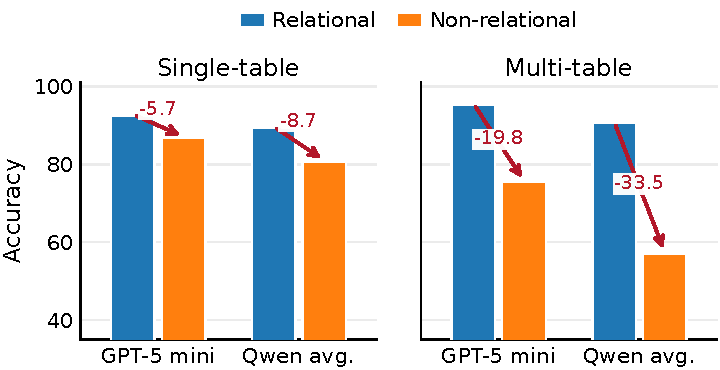
\includegraphics[width=0.48\textwidth]{img/nonrelhurts3.pdf}
    \caption{Effect of non-relational perturbations on four databases extracted from Kaggle. Bars report absolute performance under relational and non-relational variants; red arrows indicate the corresponding drop. Non-relationalization consistently degrades performance, with substantially larger drops in the multi-table setting.}
    \label{fig:nonrelhurts}
\end{figure}

\begin{figure*}[t!]
    \centering
    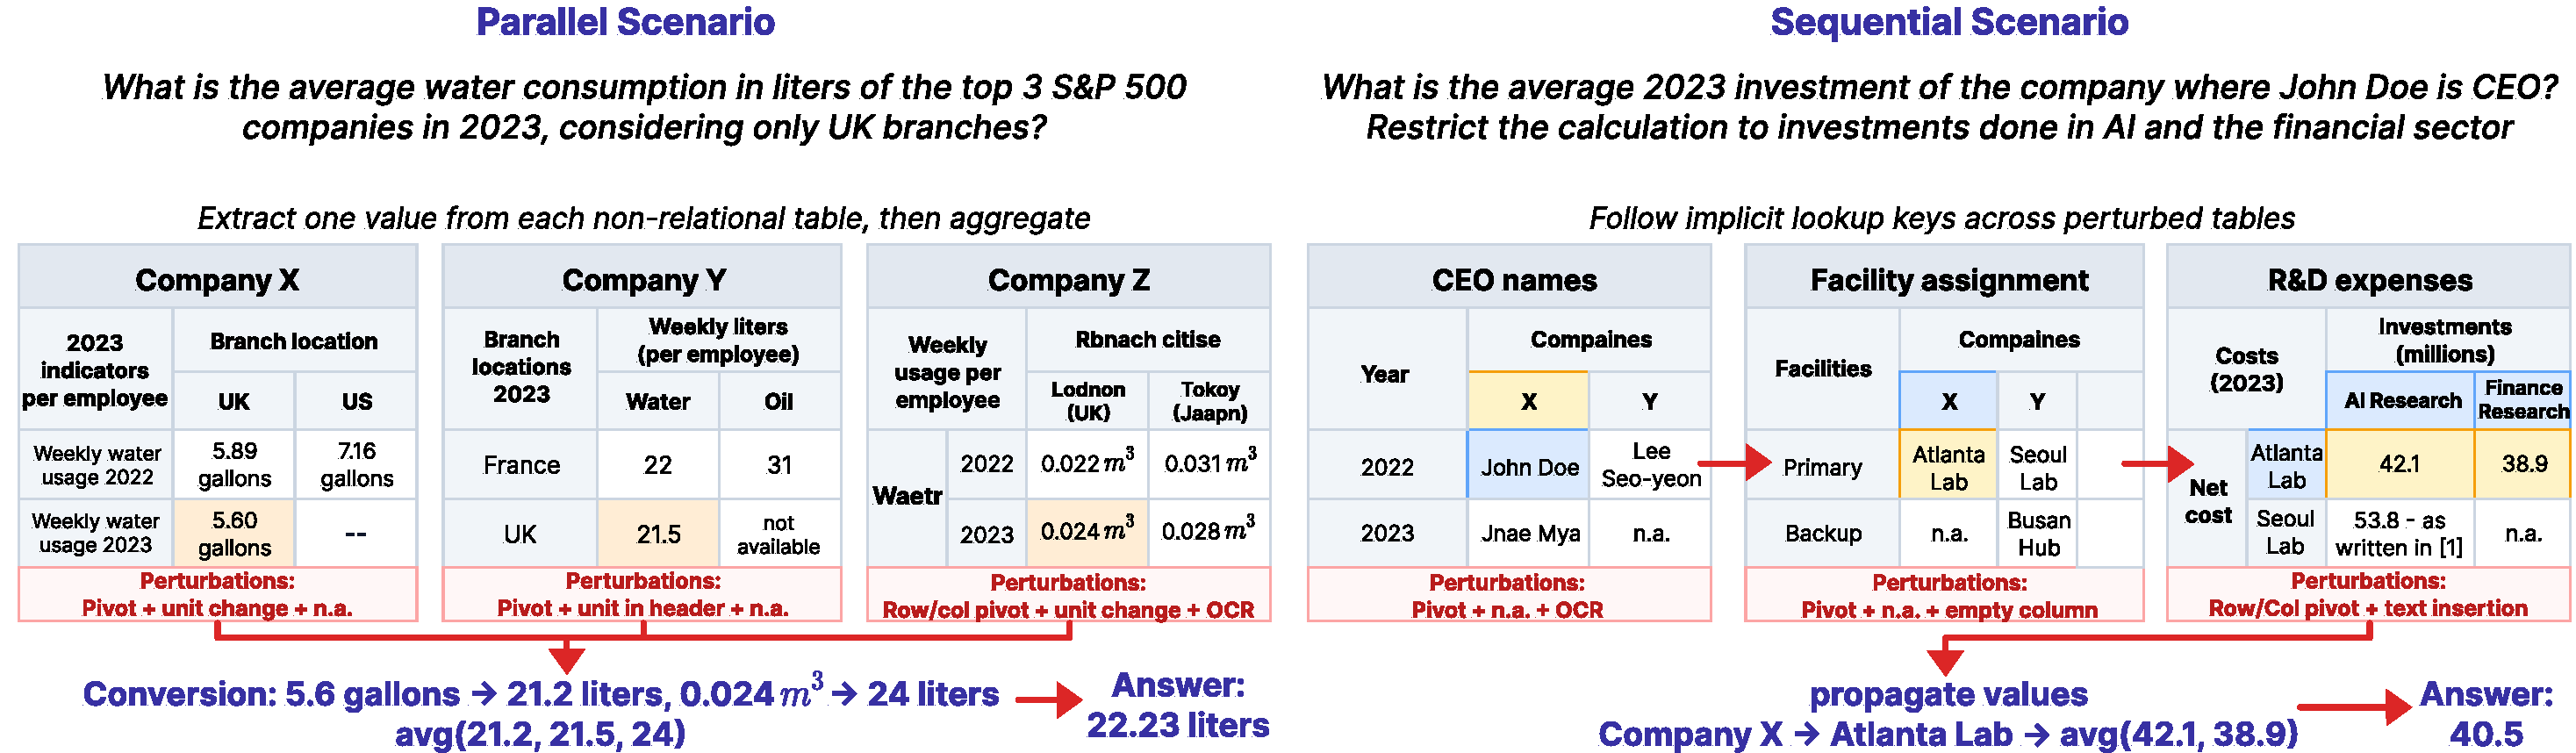
\includegraphics[width=0.99\textwidth]{img/q_types.pdf}
    \caption{Examples of parallel and sequential scenarios generated by \name over multiple non-relational tables. Parallel questions require extracting and aggregating values across perturbed tables, while sequential questions require propagating lookup keys across tables before aggregating the final values.}
    \label{fig:questiontypes}
\end{figure*}

This assumption limits the phenomena that can be evaluated. Real-world table reasoning often involves \emph{non-relational} tables with nested headers, irregular semantic links between cells, merged columns, blank rows or columns, noisy cells, and missing values. As shown in \autoref{fig:nonrelhurts}, even simple layout and cell perturbations reduce model performance, with substantially larger drops in the multi-table setting. Moreover, multi-table questions may require either recovering implicit cross-table links through semantic matching rather than foreign-key joins, which we call \emph{sequential} reasoning, or aggregating numerical evidence across many independent tables, sometimes with different units or numerical conventions, which we call \emph{parallel} reasoning. \autoref{fig:questiontypes} illustrates both regimes: the parallel example requires extracting and normalizing one water-consumption value from each company table before averaging them, while the sequential example requires identifying a company from a CEO constraint, mapping it to its main lab, and aggregating the relevant R\&D investments. Such cases naturally arise in analytical queries; for example, asking for the average CO$_2$ emissions of all S\&P 500 companies may require reasoning over hundreds of distinct tables. Existing generators do not directly target this regime, because they inherit both schemas and reasoning topology from pre-existing relational databases.

We introduce \name, a flexible \emph{from-scratch} benchmark generator for numerical question answering over multiple non-relational tables. Unlike prior work, \name~does not require an existing relational database, annotated examples, or manually curated source tables. Instead, a user specifies a target domain or topic and lightweight controls, such as the number of attributes, attribute cardinalities, number of tables, and unit settings. \name~then uses an LLM to generate a domain-specific schema, candidate attribute values, and semantic constraints, instantiates a controlled relational source table, derives executable SQL supervision with automatically verified scalar answers, and verbalizes the SQL programs into natural-language questions.

Crucially, \name~decouples correctness from presentation: answers are computed on the clean latent source, while models are evaluated on perturbed non-relational table views. From the same source, \name~constructs parallel and sequential multi-table regimes, then applies controlled structural and cell-level perturbations, including pivots, nested headers, column merging, blank rows or columns, missing values, text insertions, typos, and unit changes. Since every instance remains grounded in the latent source and executable SQL supervision, answer correctness is preserved throughout generation.

We evaluate \texttt{gpt-5-mini} and three \texttt{Qwen3.5} variants on financial and environmental instances generated by \name. Results show that performance decreases sharply as the number of tables increases, especially for parallel questions requiring many evidence values and sequential questions requiring implicit joins. We also find that unit perturbations have domain-dependent effects, suggesting that robust Table QA evaluation should account for both reasoning topology and domain-specific numerical conventions.

Finally, we show that generating comparable instances from existing real tables is difficult, since many relational tables cannot be transformed into the required non-relational layouts or multi-table reasoning structures without costly manual intervention. This motivates the from-scratch design of \name, which provides scalable control over domains, table structures, reasoning depth, and perturbations. Despite relying on synthetic tables, \name~instances are also useful for training: fine-tuning on generated data improves performance on GRI-QA \cite{1.16} compared to the non-finetuned Qwen baseline. Moreover, users can customize \name~through prompt edits, few-shot examples, manual overrides, or new perturbations matching their target application.

In summary, our contributions are threefold: (i) we introduce \name, a from-scratch generator for automatically verifiable numerical QA benchmarks over multiple non-relational tables; (ii) we define two controllable multi-table reasoning regimes, parallel and sequential, together with structural, cell-level, and unit-based perturbations that preserve answer correctness; (iii) we evaluate recent LLMs on generated financial and environmental instances, showing that non-relational perturbations, unit heterogeneity, and increasing numbers of tables substantially degrade performance, while generated instances can also improve downstream Table QA training.